\begin{frame}{Industrial Anomaly Detection: The Setting}
  \begin{columns}[T,onlytextwidth]
    \column{0.46\textwidth}
      \begin{itemize}\footnotesize\itemsep0.3em
        \item \textbf{Task:} train on defect-free images only; at test time, output an image score (accept or reject) and a pixel anomaly map. Defects are rare, and their types are not known in advance.
        \item This is the one-class case of the open-set taxonomy: its feature-distance scores now run on every image patch.
        \item \textbf{MVTec AD} (2019): 15 categories, 5,354 images, 73 defect types. \textbf{VisA} (2022): 10,821 images of 12 objects. \textbf{Real-IAD} (2024): 150K multi-view images of 30 objects.
        \item \textbf{MVTec AD 2} (2025): eight scenarios with transparent and overlapping objects, highly variable normal parts and tiny defects, each scene under at least four lighting conditions. Labels of the private test sets stay on an evaluation server.
        \item On MVTec AD and VisA, leading methods now often differ by less than one percentage point.
      \end{itemize}
    \column{0.52\textwidth}
      \centering
      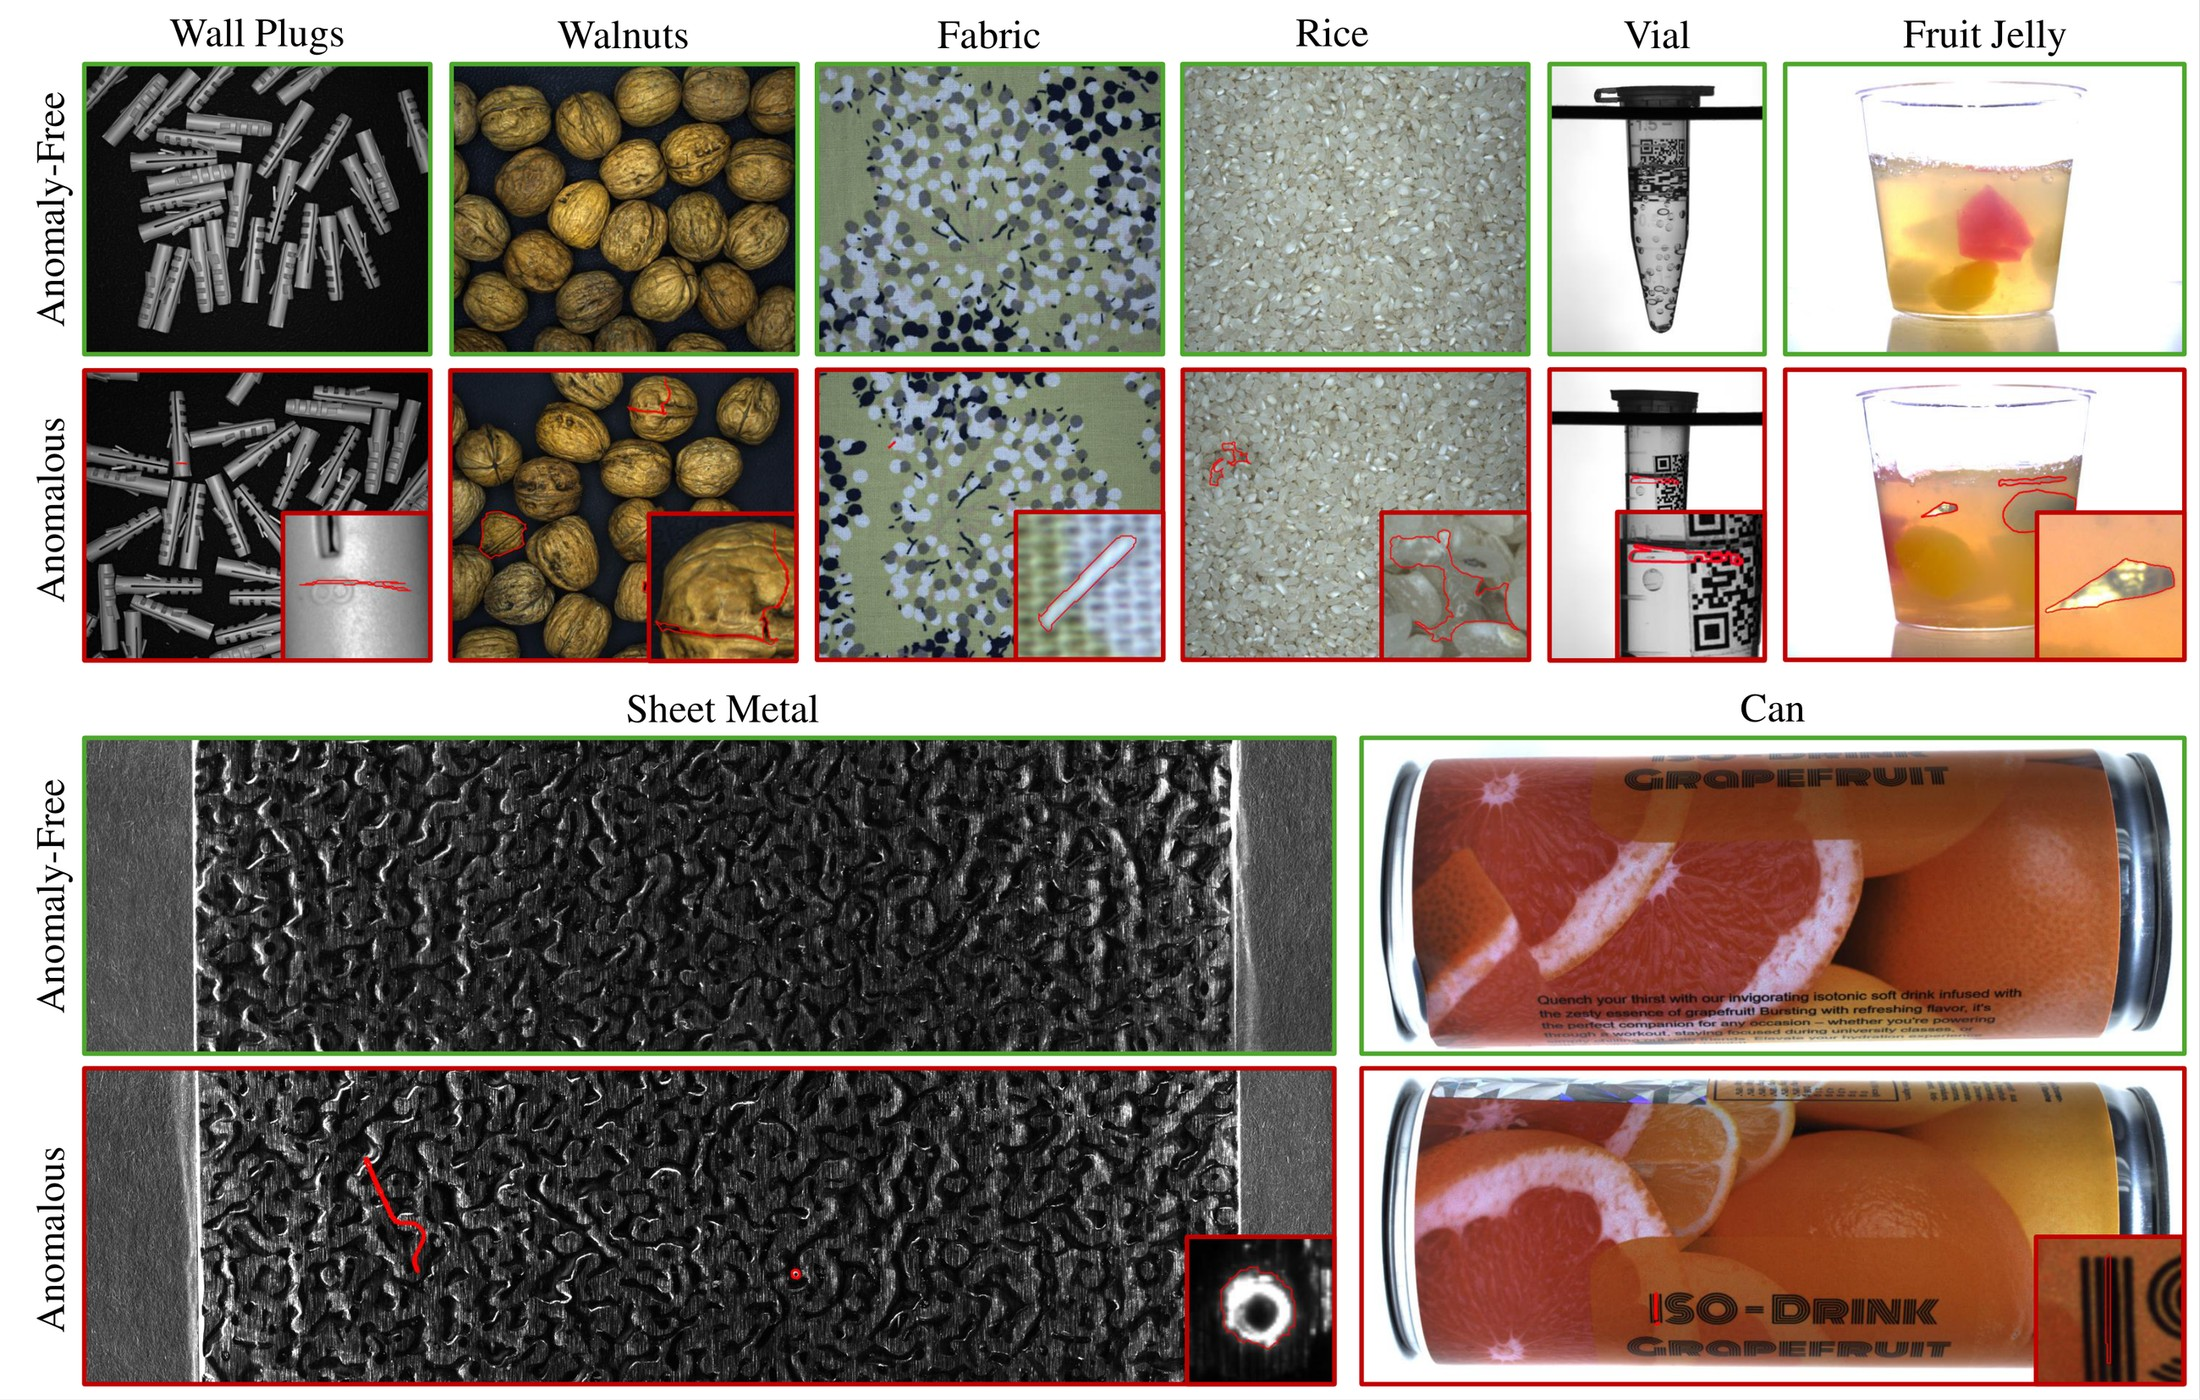
\includegraphics[width=\linewidth,height=0.62\textheight,keepaspectratio]{images/image-restoration-applications/mvtec_ad2_fig1_objects.jpg}\\[0.2em]
      {\scriptsize One defect-free (green) and one anomalous (red) image per object. Heckler-Kram et al., ``The MVTec AD 2 Dataset: Advanced Scenarios for Unsupervised Anomaly Detection,'' 2025, \href{https://arxiv.org/abs/2503.21622v1}{arXiv:2503.21622v1}, Figure~1.\par}
  \end{columns}
\end{frame}

\begin{frame}{Scoring Pixels: Pixel AUROC Versus PRO}
  \begin{columns}[T,onlytextwidth]
    \column{0.52\textwidth}
      \begin{itemize}\footnotesize\itemsep0.3em
        \item \textbf{Pixel AUROC} is AUROC over all test pixels. Normal pixels dominate (97.26\% of MVTec AD, 99.45\% of VisA), so a high value says little: on Real-IAD, Dinomaly reaches 98.8\% pixel AUROC but 89.3\% image AUROC.
        \item \textbf{Per-region overlap (PRO)} weights every defect region equally:
        \[ \mathrm{PRO}(t) = \frac{1}{K}\sum_{i}\sum_{j=1}^{k_i}\frac{|P_t \cap C_{i,j}|}{|C_{i,j}|} \]
        $C_{i,j}$: the $j$-th connected defect region of test image $i$; $P_t$: pixels flagged at threshold $t$; $K=\sum_i k_i$: number of regions.
        \item \textbf{AU-PRO} integrates PRO over the pixel false-positive rate (FPR) up to 0.3, normalised. Methods above 90\% on MVTec AD reach at most 58.7\% on MVTec AD 2; at its stricter limit of 0.05 (AU-PRO\textsubscript{0.05}) the best mean is 30.8\% (EfficientAD).
      \end{itemize}
    \column{0.46\textwidth}
      \centering
      \vspace{0.6em}
      \resizebox{\linewidth}{!}{%
      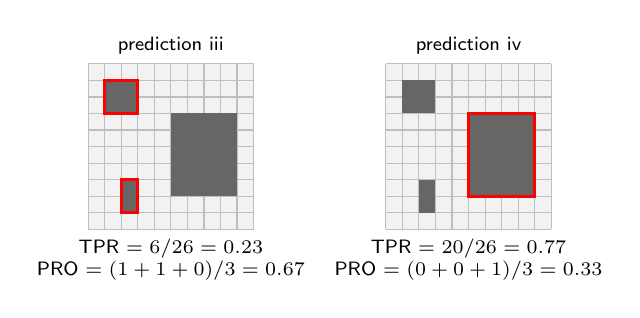
\begin{tikzpicture}[x=0.21cm, y=0.21cm, font=\sffamily\scriptsize]
        \foreach \ox/\lab in {0/{prediction iii}, 18/{prediction iv}} {
          \fill[black!5] (\ox,0) rectangle (\ox+10,10);
          \draw[black!25, step=1] (\ox,0) grid (\ox+10,10);
          \fill[black!60] (\ox+1,7) rectangle (\ox+3,9);
          \fill[black!60] (\ox+5,2) rectangle (\ox+9,7);
          \fill[black!60] (\ox+2,1) rectangle (\ox+3,3);
          \node[above] at (\ox+5,10) {\lab};
        }
        \draw[red, line width=1.2pt] (1,7) rectangle (3,9);
        \draw[red, line width=1.2pt] (2,1) rectangle (3,3);
        \draw[red, line width=1.2pt] (23,2) rectangle (27,7);
        \node[below, align=center] at (5,0) {TPR $=6/26=0.23$\\PRO $=(1+1+0)/3=0.67$};
        \node[below, align=center] at (23,0) {TPR $=20/26=0.77$\\PRO $=(0+0+1)/3=0.33$};
      \end{tikzpicture}}\\[0.4em]
      {\scriptsize Three defects of 4, 20 and 2 pixels (grey); red outlines mark the pixels a thresholded map flags. The pixel true-positive rate (TPR) favours the large defect; PRO counts each defect once. Redrawn after Heckler-Kram et al., \href{https://arxiv.org/abs/2503.21622v1}{arXiv:2503.21622v1}, Figure~4 (cases iii and iv). Normal-pixel shares: Li et al. (MuSc), \href{https://arxiv.org/abs/2401.16753v1}{arXiv:2401.16753v1}, Sec.~1.\par}
  \end{columns}
\end{frame}

\begin{frame}{From Reconstruction to Patch Memory: PatchCore}
  \begin{itemize}\footnotesize\itemsep0.2em
    \item Reconstruction models fail both ways: they blur fine normal texture (false alarms), and they learn to rebuild anomalies too, the identity shortcut (missed defects). Feature-space methods compare frozen ImageNet-backbone features instead.
    \item \textbf{PaDiM} fits one Gaussian $\mathcal{N}(\mu_{ij},\Sigma_{ij})$ per patch position $(i,j)$ over the normal images and scores a test patch by its Mahalanobis distance.
    \item \textbf{PatchCore} pools the mid-level patch features of all normal images into a memory bank $\mathcal{M}$, keeps a greedy coreset (1--25\% of $\mathcal{M}$, chosen so every stored feature has a close representative), and scores each test patch by its nearest-neighbour distance. The image score is the largest patch score, re-weighted by how isolated its nearest memory feature is.
    \item MVTec AD: image AUROC 99.1\% (PaDiM 97.9\%), pixel AUROC 98.1\%, PRO 93.4\%; 42 of 1,725 test images misclassified.
  \end{itemize}
  \centering
  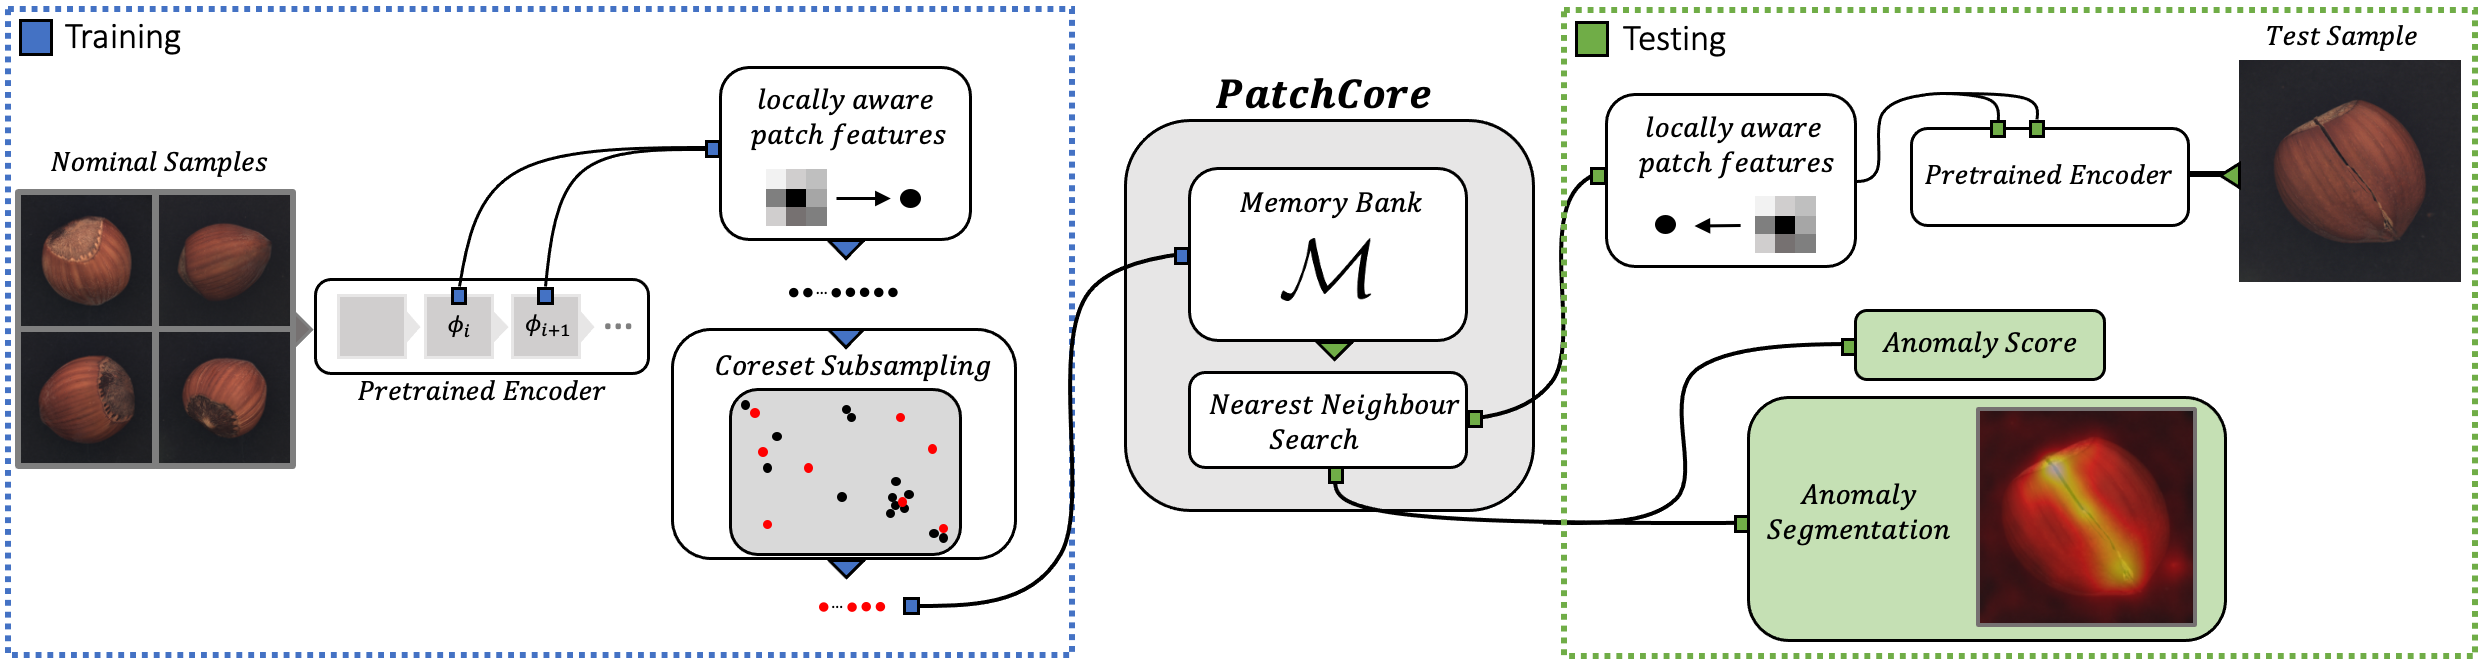
\includegraphics[width=\textwidth,height=0.23\textheight,keepaspectratio]{images/image-restoration-applications/patchcore_fig2_overview.png}\\[0.1em]
  {\scriptsize Roth et al., ``Towards Total Recall in Industrial Anomaly Detection,'' CVPR 2022, \href{https://arxiv.org/abs/2106.08265v2}{arXiv:2106.08265v2}, Figure~2.}
\end{frame}

\begin{frame}{EfficientAD: A Millisecond Student-Teacher}
  \begin{itemize}\footnotesize\itemsep0.2em
    \item \textbf{Student-teacher} detection (Bergmann et al., 2020): a student learns to reproduce a frozen teacher's features on normal images only; where the two disagree, the input is unfamiliar.
    \item The teacher is a four-layer \textbf{patch description network} (PDN) distilled from WideResNet-101 features; each output vector sees one 33$\times$33 patch. A hard feature loss trains the student only on the 0.1\% of outputs where it is worst.
    \item \textbf{Logical anomalies} (a missing, extra or misplaced part) need the whole image: an autoencoder predicts the teacher's features through a 64-number bottleneck; where the student disagrees with it, the global map lights up.
    \item Mean over MVTec AD, VisA and MVTec LOCO (a logical-anomaly benchmark): EfficientAD-S 95.4\% image AUROC at 2.2\,ms per image; PatchCore 91.1\% at 32\,ms (RTX A6000).
  \end{itemize}
  \centering
  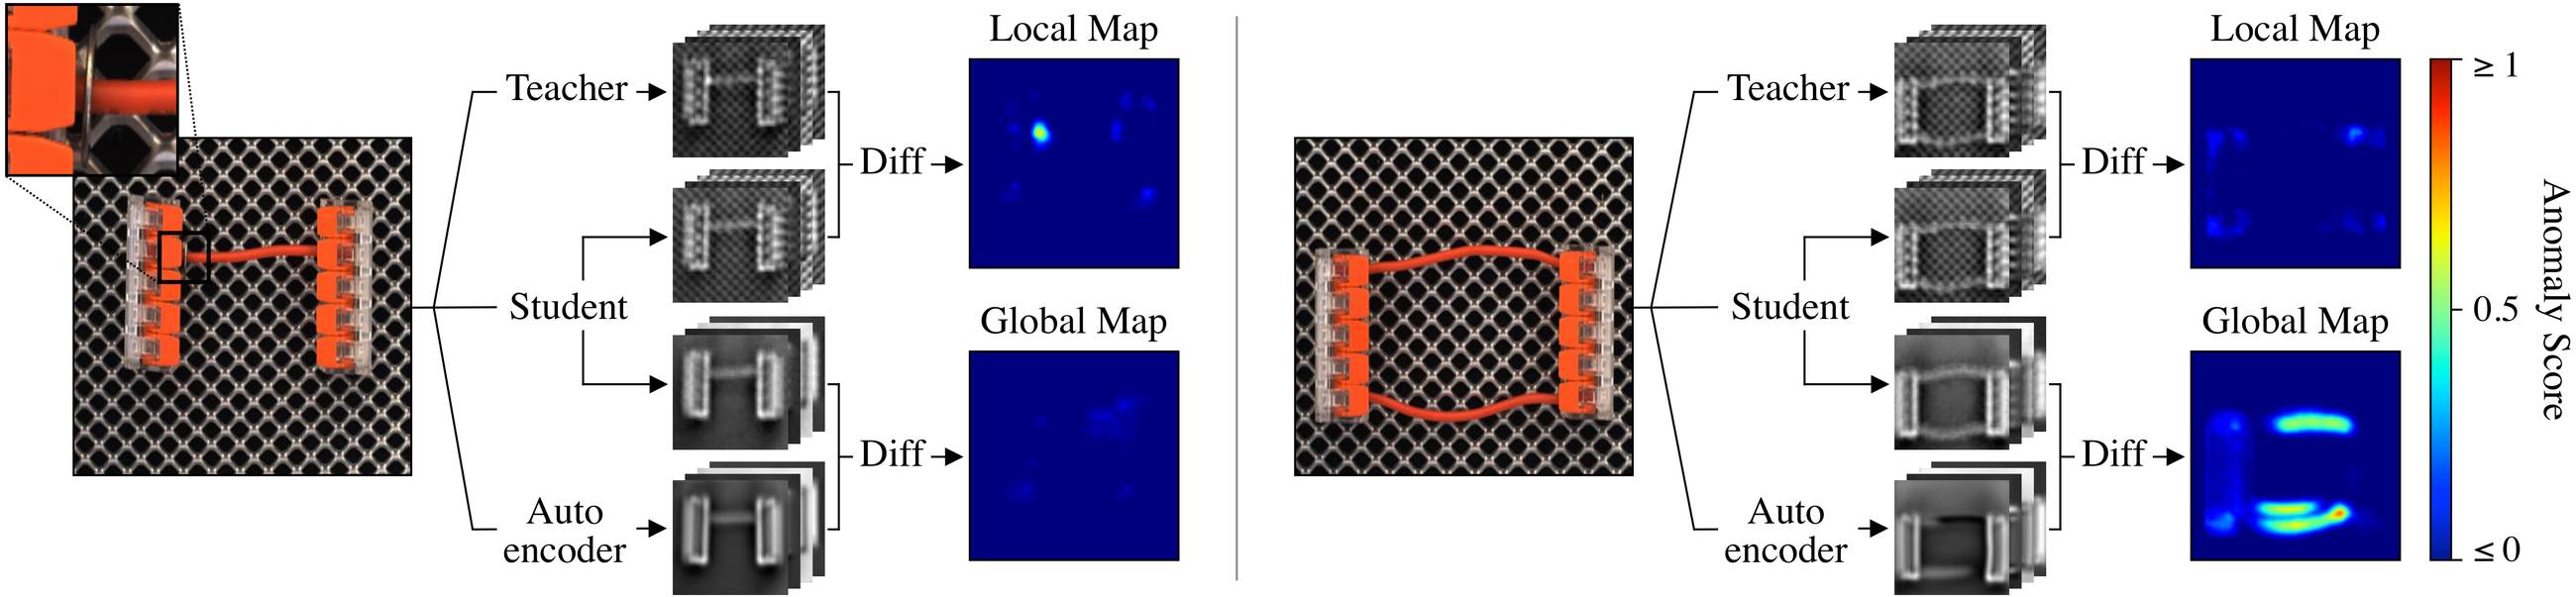
\includegraphics[width=\textwidth,height=0.25\textheight,keepaspectratio]{images/image-restoration-applications/efficientad_fig5_student_teacher_autoencoder.png}\\[0.1em]
  {\scriptsize A washer at the cable end shows in the local map (left); a second cable shows only in the global map (right). Batzner et al., ``EfficientAD: Accurate Visual Anomaly Detection at Millisecond-Level Latencies,'' WACV 2024, \href{https://arxiv.org/abs/2303.14535v3}{arXiv:2303.14535v3}, Figure~5.\par}
\end{frame}

\begin{frame}{Dinomaly: One Model for Every Category}
  \begin{columns}[T,onlytextwidth]
    \column{0.44\textwidth}
      \begin{itemize}\footnotesize\itemsep0.3em
        \item \textbf{One model, all products.} Unified models trailed per-class ones: diverse normal data teaches a decoder to copy its input. The best earlier unified model reached 98.6\% image AUROC on MVTec AD.
        \item A plain Transformer decoder rebuilds the features of a frozen DINOv2 ViT-B/14 with registers; the anomaly map is their cosine distance.
        \item \textbf{Noisy bottleneck:} dropout (rate 0.2; 0.4 on Real-IAD) in the MLP between encoder and decoder corrupts what the decoder receives.
        \item \textbf{Linear attention}, whose cost grows linearly with the number of tokens, spreads over the whole image, so the decoder cannot copy the query position.
        \item \textbf{Loose reconstruction:} match groups of layers, and scale down the gradient of points that are already rebuilt well.
      \end{itemize}
    \column{0.54\textwidth}
      \centering
      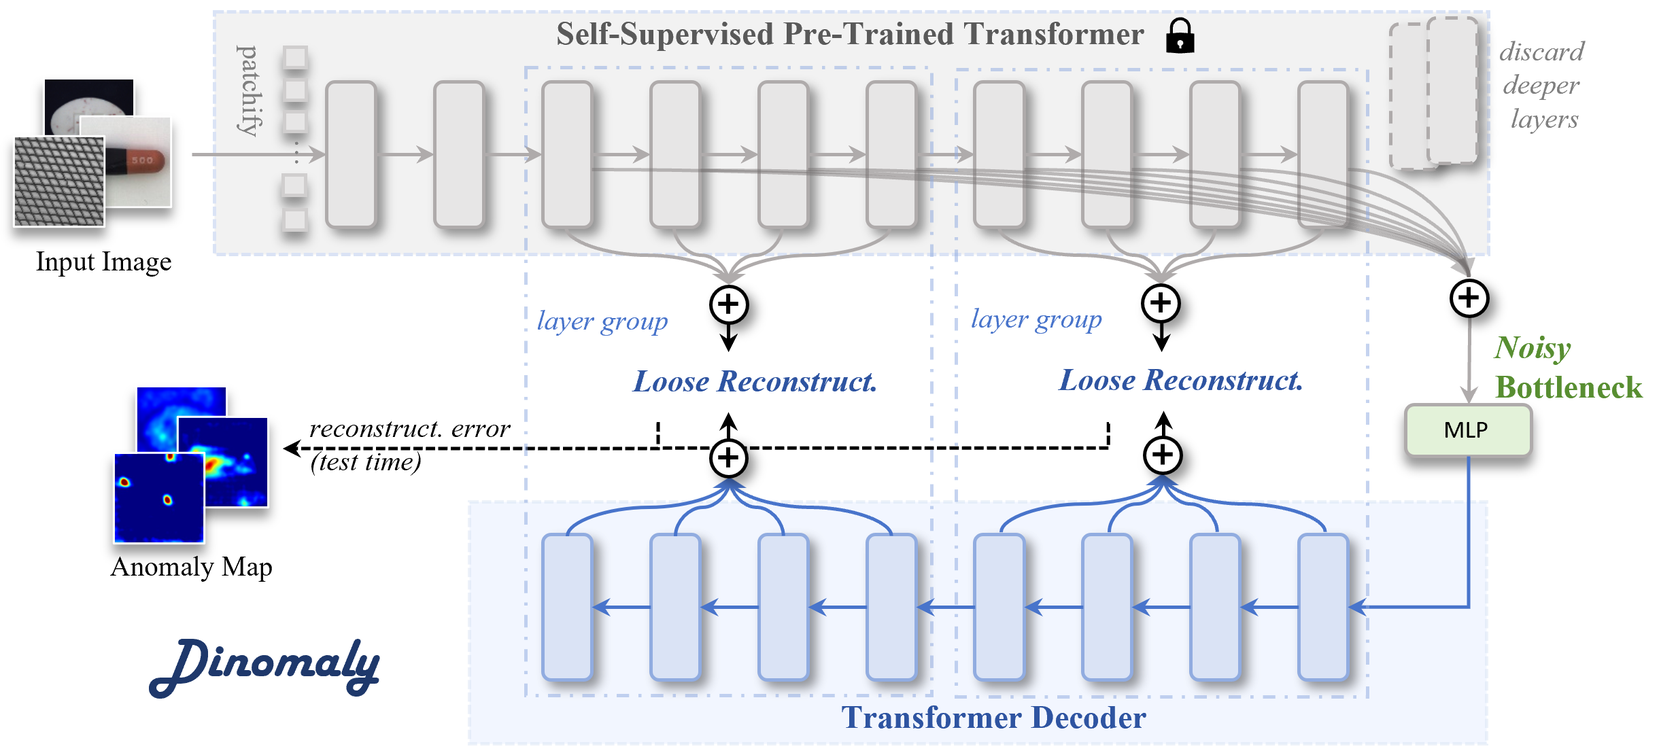
\includegraphics[width=\linewidth,height=0.46\textheight,keepaspectratio]{images/image-restoration-applications/dinomaly_fig2_pipeline.png}\\[0.1em]
      {\scriptsize Guo et al., ``Dinomaly: The Less Is More Philosophy in Multi-Class Unsupervised Anomaly Detection,'' CVPR 2025, \href{https://arxiv.org/abs/2405.14325v5}{arXiv:2405.14325v5}, Figure~2 (left part).\par}
      \vspace{0.5em}
      {\scriptsize
      \begin{tabular}{l c c c}
        \toprule
        \textbf{Dataset} & \textbf{Image} & \textbf{Pixel} & \textbf{AU-PRO} \\
        \midrule
        MVTec AD & 99.6 & 98.4 & 94.8 \\
        VisA & 98.7 & 98.7 & 94.5 \\
        Real-IAD & 89.3 & 98.8 & 93.9 \\
        \bottomrule
      \end{tabular}\par}
      {\scriptsize One model per dataset for all its categories: image and pixel AUROC and AU-PRO (\%). Guo et al., Table~1.\par}
  \end{columns}
\end{frame}

\begin{frame}{Foundation Models: Zero- and Few-Shot Detection}
  \begin{columns}[T,onlytextwidth]
    \column{0.50\textwidth}
      \begin{itemize}\footnotesize\itemsep0.3em
        \item \textbf{WinCLIP} compares each image with CLIP prompt ensembles such as ``a cropped photo of the flawless [object]'' against ``damaged'' variants; sliding windows of patches give the map. WinCLIP+ adds patches from a few normal images.
        \item \textbf{AnomalyCLIP} learns CoOp-style prompts with the class name replaced by the word ``object'', trained once on another labelled dataset, so they encode normal versus damaged for any product.
        \item \textbf{AnomalyDINO} trains nothing: DINOv2 patch features of 1--16 normal images form the memory bank, scored by nearest-neighbour distance as in PatchCore.
        \item \textbf{MuSc} needs neither prompts nor normal images: normal patches find many look-alikes in the other unlabelled test images, defects find few. It requires a batch of test images.
      \end{itemize}
    \column{0.48\textwidth}
      \centering
      \vspace{0.8em}
      {\scriptsize
      \begin{tabular}{l >{\raggedright\arraybackslash}p{2.1cm} c c}
        \toprule
        \textbf{Method} & \textbf{Needs at test time} & \textbf{Image} & \textbf{Pixel} \\
        \midrule
        WinCLIP & text prompts & 91.8 & 85.1 \\
        AnomalyCLIP & prompts trained on VisA & 91.5 & 91.1 \\
        MuSc & the unlabelled test set & 97.8 & 97.3 \\
        \addlinespace[0.25em]
        WinCLIP+ & one normal image & 93.1 & 95.2 \\
        AnomalyDINO & one normal image & 96.6 & 96.8 \\
        \addlinespace[0.25em]
        PatchCore & all normal training images & 99.1 & 98.1 \\
        \bottomrule
      \end{tabular}\par}
      \vspace{0.4em}
      {\scriptsize MVTec AD image and pixel AUROC (\%), from each paper: Jeong et al., CVPR 2023, \href{https://arxiv.org/abs/2303.14814v1}{arXiv:2303.14814v1}; Zhou et al., ICLR 2024, \href{https://arxiv.org/abs/2310.18961v12}{arXiv:2310.18961v12}, Table~1; Li et al., ICLR 2024, \href{https://arxiv.org/abs/2401.16753v1}{arXiv:2401.16753v1}, Table~1; Damm et al., WACV 2025, \href{https://arxiv.org/abs/2405.14529v3}{arXiv:2405.14529v3}, Table~2; Roth et al., Tables~1--2.\par}
  \end{columns}
\end{frame}

\begin{frame}{Multimodal LLMs as Inspectors}
  \begin{columns}[T,onlytextwidth]
    \column{0.52\textwidth}
      \begin{itemize}\footnotesize\itemsep0.3em
        \item \textbf{AnomalyGPT} (2024): a decoder matches image patches against ``normal'' and ``abnormal'' text to localise, and a prompt learner passes the map to a frozen multimodal LLM (MLLM); only the decoder and prompt learner are trained, on simulated defects. With one normal image: 94.1\% image and 95.3\% pixel AUROC on MVTec AD, and a verdict with no hand-set threshold.
        \item \textbf{MMAD} (2025): 39,672 multiple-choice questions on 8,366 industrial images, over seven subtasks (is it defective, which defect, where, describe it, analyse it, and two about the object), each with one normal template image.
        \item Showing InternVL2-40B the maps of PatchCore or AnomalyCLIP mostly helped only the ``where'' answers and hurt the rest, since detectors also mark normal images; ground-truth boxes improved all four measured subtasks. The quality of the localisation map limits what the MLLM can answer.
      \end{itemize}
    \column{0.46\textwidth}
      \centering
      \vspace{0.6em}
      {\scriptsize\setlength{\tabcolsep}{4pt}
      \begin{tabular}{l c c c}
        \toprule
        \textbf{Model} & \textbf{Defective?} & \textbf{Where?} & \textbf{Mean of 7} \\
        \midrule
        Random choice & 50.0 & 25.0 & 28.6 \\
        AnomalyGPT (7B) & 65.6 & 28.0 & 36.5 \\
        InternVL2 (76B) & 68.3 & 56.7 & 70.8 \\
        GPT-4o & 68.6 & 55.6 & 74.9 \\
        \addlinespace[0.25em]
        Non-experts & 86.9 & 85.6 & 78.7 \\
        Experts & 95.2 & 92.3 & 86.7 \\
        \bottomrule
      \end{tabular}\par}
      \vspace{0.4em}
      {\scriptsize MMAD accuracy (\%). Human scores from a 177-question study (3 anomaly-detection researchers, 5 non-experts). Jiang et al., ``MMAD: A Comprehensive Benchmark for Multimodal Large Language Models in Industrial Anomaly Detection,'' ICLR 2025, \href{https://arxiv.org/abs/2410.09453v3}{arXiv:2410.09453v3}, Table~2 and Figure~6; Gu et al., AAAI 2024, \href{https://arxiv.org/abs/2308.15366v4}{arXiv:2308.15366v4}.\par}
  \end{columns}
\end{frame}

\begin{frame}{From Benchmark to Production Line}
  \begin{columns}[T,onlytextwidth]
    \column{0.49\textwidth}
      \begin{itemize}\footnotesize\itemsep0.3em
        \item \textbf{Known defect types:} when labelled examples exist, a supervised detector or segmenter is the right tool; the one-class model covers defects nobody has seen yet.
        \item \textbf{Few defect images:} synthesise more. DRAEM pastes textures inside random Perlin-noise shapes on normal images and trains a network to segment them. AnomalyDiffusion keeps a latent diffusion model frozen and learns one textual-inversion embedding per defect type from a third of MVTec AD's real defects; a U-Net trained on 1,000 generated image-mask pairs per type reaches 99.1\% pixel AUROC.
        \item \textbf{Thresholds from normal data only:} MVTec AD 2's baseline flags pixels above the mean plus three standard deviations of defect-free validation scores; there PatchCore's mean pixel F1 is 3.7\% against MSFlow's 21.8\%, at similar AU-PRO.
      \end{itemize}
    \column{0.49\textwidth}
      \begin{itemize}\footnotesize\itemsep0.3em
        \item \textbf{Resolution costs time:} on MVTec AD 2's rice scenario, the largest input roughly doubles PatchCore's AU-PRO\textsubscript{0.05}, but inference takes 2\,s per image on an RTX 2080 Ti.
        \item \textbf{Lighting shift:} MSFlow, a detector built on normalizing flows, drops from 24.3\% to 11.9\% AU-PRO\textsubscript{0.05} under changed illumination; a reverse-distillation student-teacher (RD) loses 1.4 points.
        \item \textbf{Runs locally:} Intel's open-source anomalib library (Apache-2.0; release 2.6.2, September 2026) implements PaDiM, PatchCore, EfficientAD, Dinomaly, WinCLIP and AnomalyDINO among 30 image models; most export to OpenVINO for Intel CPUs and GPUs.
      \end{itemize}
  \end{columns}
  {\scriptsize DRAEM: \href{https://arxiv.org/abs/2108.07610v2}{arXiv:2108.07610v2}; AnomalyDiffusion: \href{https://arxiv.org/abs/2312.05767v2}{arXiv:2312.05767v2}; MVTec AD 2: \href{https://arxiv.org/abs/2503.21622v1}{arXiv:2503.21622v1}, Sec.~4, Tables~7--8, Figure~6; \href{https://github.com/open-edge-platform/anomalib}{anomalib}.\par}
\end{frame}
